% !TEX program = xelatex
\documentclass[12pt, a4paper]{article}

% ============ 中文支持 ============
\usepackage[UTF8, heading=true]{ctex}
\setCJKmainfont{SimSun}
\setCJKsansfont{SimHei}

% ============ 页面与排版 ============
\usepackage[margin=2.5cm]{geometry}
\usepackage{setspace}
\onehalfspacing
\usepackage{parskip}
\setlength{\parskip}{0.3em}

% ============ 图表 ============
\usepackage{graphicx}
\graphicspath{{../image/report/}}
\usepackage{float}
\usepackage{booktabs}
\usepackage{multirow}
\usepackage{longtable}
\usepackage{tabularx}
\usepackage{caption}
\captionsetup{font=small, labelfont=bf, labelsep=quad}
\captionsetup[lstlisting]{name=代码清单}

% ============ 数学 ============
\usepackage{amsmath, amssymb}

% ============ 代码 ============
\usepackage{listings}
\usepackage{xcolor}
\lstset{
  basicstyle=\small\ttfamily,
  backgroundcolor=\color{gray!8},
  frame=single,
  breaklines=true,
  numbers=left,
  numberstyle=\tiny\color{gray},
  keywordstyle=\color{blue!70!black}\bfseries,
  commentstyle=\color{green!50!black},
  stringstyle=\color{orange!70!black},
  showstringspaces=false,
  tabsize=2,
  literate={—}{{\textemdash}}1,
}

% ============ 链接 ============
\usepackage[colorlinks=true, linkcolor=blue!70!black, citecolor=green!50!black, urlcolor=blue!60!black]{hyperref}

% ============ 页眉页脚 ============
\usepackage{fancyhdr}
\pagestyle{fancy}
\fancyhf{}
\fancyhead[L]{\small 人工智能实验}
\fancyhead[R]{\small 团队大作业报告}
\fancyfoot[C]{\thepage}
\renewcommand{\headrulewidth}{0.4pt}

% ============ 标题信息 ============
\title{\textbf{人脸识别系统的设计与实现}}
\author{
  程锦帅、牛艺卓、段炫亿、陈俊宇 \\
  \textit{人工智能实验 · 团队大作业}
}
\date{2026年6月}

\begin{document}

% ============ 封面 ============
\begin{titlepage}
\centering
\vspace*{3cm}
{\Huge\bfseries 团队大作业报告\par}
{\Large 人工智能实验2026年春季学期\par}
\vspace{1.5cm}
{\Huge\bfseries 题目：人脸识别系统的设计与实现\par}
\vspace{2cm}
{\large
\begin{tabular}{rl}
\textbf{组员：} & 程锦帅（项目统筹、代码实现、前端开发、报告撰写） \\
               & 牛艺卓（数据收集、标注质量审查、辅助报告撰写） \\
               & 段炫亿（数据收集、数据标注、辅助前端开发） \\
               & 陈俊宇（数据收集、数据标注、演示视频录制） \\
\end{tabular}
}
\vfill
{\large 2026年6月\par}
\end{titlepage}

% ============ 目录 ============
% \newpage
% \tableofcontents

% ============ 正文 ============
\newpage

% ======== 第二章 ========
\section{数据收集与标注}

\subsection{数据来源}

该作业的数据集分为两部分：

\begin{itemize}
  \item \textbf{CelebA数据集}：来源于 CelebA，选取 100 类身份，每类 3 张注册图、3 张测试图，共 600 张图片。该数据集已经由老师给出。
  \item \textbf{自收集20类数据集}：按要求收集 20 位公开人物的照片数据，涵盖影视、音乐、体育、政治、科学、商业等领域，包括中外名人。数据来源为互联网公开图片，通过搜索引擎按人物姓名检索获取。小组成员收集时注意选择光照条件各异、拍摄角度不同、背景多变的图片，以模拟真实应用场景。
\end{itemize}

\subsection{数据集划分}

自收集数据集中，每位人物收集 5 张照片，按以下规则划分：

\begin{table}[H]
\centering
\caption{自收集数据集划分}
\label{tab:dataset-split}
\begin{tabular}{cccc}
\toprule
划分 & 每人数量 & 总计 & 用途 \\
\midrule
注册集 & 2 张 & 40 张 & 构建身份底库 \\
测试集 & 3 张 & 60 张 & 评测识别准确率 \\
\bottomrule
\end{tabular}
\end{table}

测试集的 3 张图片包含：1 张单人照（仅包含目标人物）和 2 张多人照（包含目标人物及其他人员）。注册集与测试集无重复图片，测试集不参与底库构建或任何训练过程。

\subsection{数据集目录结构}

自收集数据集的目录组织如下：

\begin{lstlisting}[language={}, caption={数据集目录结构}, label={lst:dataset-structure}]
dataset/
+-- identities.csv              # 身份映射表
+-- annotations.jsonl           # 测试集标注文件
+-- registered/                 # 注册集
|   +-- p01/
|   |   +-- p01_r01.jpg/png
|   |   +-- p01_r02.jpg/png
|   +-- ... (p02 ~ p20)
+-- test/                       # 测试集
    +-- images/
        +-- p01_t01.jpg/png     # 单人照
        +-- p01_t02.jpg/png     # 多人照
        +-- p01_t03.jpg/png     # 多人照
        +-- ... (p02 ~ p20)
\end{lstlisting}

\subsection{标注格式}

测试集采用文档中要求的 \texttt{annotations.jsonl} 格式进行标注，每行对应一张测试图片的完整标注信息。标注字段说明如下：

\begin{itemize}
  \item \texttt{image}：图片相对路径
  \item \texttt{image\_type}：图片类型，\texttt{single} 表示单人照，\texttt{multi} 表示多人照
  \item \texttt{faces}：人脸列表，每个人脸包含：
  \begin{itemize}
    \item \texttt{identity\_id}：身份编号（p01\~{}p20 为已知身份，\texttt{unknown} 为非目标身份人员）
    \item \texttt{bbox}：边界框坐标 $[x, y, w, h]$，采用绝对像素坐标，原点为图片左上角
  \end{itemize}
\end{itemize}

多人照标注规则：清晰可见的人脸全部标注，属于 20 类目标身份的人物填写对应的 \texttt{identity\_id}，不属于目标身份的人员统一填写 \texttt{unknown}。

以下为标注文件中的实际样例数据：

单人照标注（\texttt{p01\_t01.jpg}，仅含目标人物成龙）：
\begin{lstlisting}[language={}, caption={单人照标注样例}, label={lst:ann-single}]
{"image":"test/images/p01_t01.jpg","image_type":"single",
 "faces":[{"identity_id":"p01","bbox":[125,62,223,309]}]}
\end{lstlisting}

多人照标注（\texttt{p01\_t02.jpg}，含目标人物及其他人员，目标人物置于首位）：
\begin{lstlisting}[language={}, caption={多人照标注样例}, label={lst:ann-multi}]
{"image":"test/images/p01_t02.png","image_type":"multi",
 "faces":[{"identity_id":"p01","bbox":[298,87,85,101]},
           {"identity_id":"unknown","bbox":[475,59,82,107]},
           {"identity_id":"unknown","bbox":[85,74,62,100]}]}
\end{lstlisting}

图~\ref{fig:sample-single} 和图~\ref{fig:sample-multi} 分别展示了单人照和多人照的数据样例。

\begin{figure}[H]
  \centering
  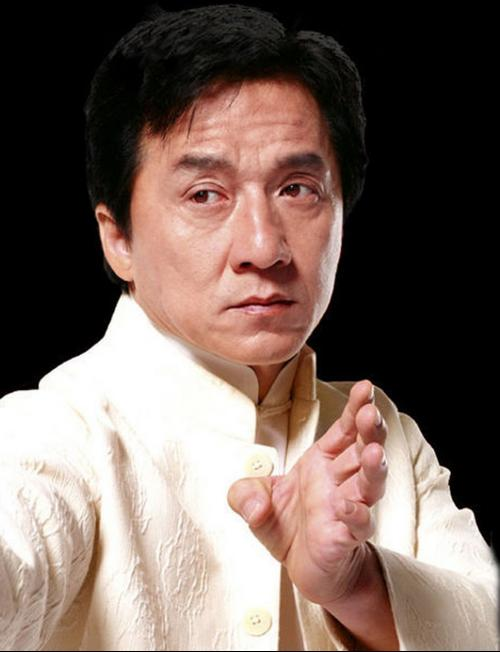
\includegraphics[width=0.4\textwidth]{p01_t01_sample.jpg}
  \caption{单人照样例：p01\_t01.jpg（成龙）}
  \label{fig:sample-single}
\end{figure}

\begin{figure}[H]
  \centering
  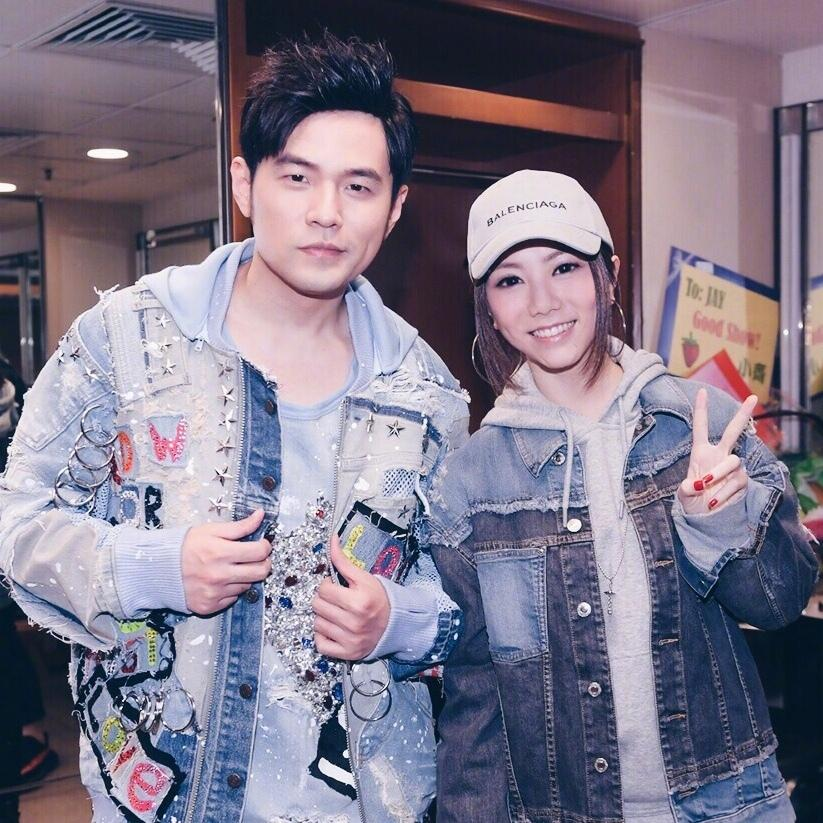
\includegraphics[width=0.6\textwidth]{p05_t02_sample.jpg}
  \caption{多人照样例：p05\_t02.jpg（邓紫棋与周杰伦）}
  \label{fig:sample-multi}
\end{figure}

\subsection{身份映射表}

自收集数据集映射关系如表~\ref{tab:identities} 所示。

\begin{table}[H]
\centering
\caption{身份映射表（20 类公开人物）}
\label{tab:identities}
\begin{tabular}{cccc}
\toprule
identity\_id & 人物姓名 & 领域 & 类别 \\
\midrule
p01 & 成龙 & 影视 & 中国 \\
p02 & 章子怡 & 影视 & 中国 \\
p03 & 刘德华 & 影视/音乐 & 中国 \\
p04 & 周杰伦 & 音乐 & 中国 \\
p05 & 邓紫棋 & 音乐 & 中国 \\
p06 & 姚明 & 体育 & 中国 \\
p07 & 谷爱凌 & 体育 & 中国 \\
p08 & 郎平 & 体育 & 中国 \\
p09 & 马云 & 商业/科技 & 中国 \\
p10 & 屠呦呦 & 科学 & 中国 \\
p11 & Barack Obama & 政治 & 国际 \\
p12 & Angela Merkel & 政治 & 国际 \\
p13 & Narendra Modi & 政治 & 国际 \\
p14 & Jacinda Ardern & 政治 & 国际 \\
p15 & Taylor Swift & 音乐 & 国际 \\
p16 & Beyoncé & 音乐 & 国际 \\
p17 & Dwayne Johnson & 影视 & 国际 \\
p18 & Emma Watson & 影视 & 国际 \\
p19 & Lionel Messi & 体育 & 国际 \\
p20 & Serena Williams & 体育 & 国际 \\
\bottomrule
\end{tabular}
\end{table}


% ======== 第三章 ========
\section{模型与系统实现}

\subsection{模型选择与原理}

本系统采用 MTCNN + InceptionResnetV1 的人脸识别方案，由人脸检测和特征提取两个模块组成。

\subsubsection{人脸检测：MTCNN}

MTCNN（Multi-task Cascaded Convolutional Networks）是由 Zhang 等人\cite{zhang2016mtcnn}于 2016 年提出的人脸检测算法，采用三级级联架构逐级精化检测结果：

\textbf{第一级 PNet（Proposal Network）：}输入为经过多尺度缩放的图片金字塔，通过轻量级卷积网络快速扫描整张图片，生成大量候选人脸区域。PNet 同时输出每个候选区域的人脸分类得分和边界框回归偏移量，通过非极大值抑制（NMS）过滤重叠度高的候选框。该级网络参数极少（约 6,600 个），能够快速处理大尺度图片。

\textbf{第二级 RNet（Refine Network）：}将 PNet 输出的候选区域裁剪并缩放为 $24 \times 24$ 像素，送入更复杂的卷积网络进行精细判断。RNet 进一步过滤误检区域，并对边界框进行更精确的回归。相比 PNet，RNet 增加了全连接层，参数量约 100,000 个，分类准确率显著提升。

\textbf{第三级 ONet（Output Network）：}将 RNet 输出的候选区域裁剪缩放为 $48 \times 48$ 像素，送入最深层的卷积网络。ONet 不仅输出最终的人脸分类得分和边界框坐标，还回归 5 个面部关键点位置（左眼、右眼、鼻尖、左嘴角、右嘴角），用于后续的人脸对齐。ONet 参数量约 389,000 个。

本系统使用的 MTCNN 总参数量约 0.5M，设置 \texttt{min\_face\_size=20}（最小检测人脸尺寸 20 像素）以适应不同分辨率的输入图片，设置 \texttt{keep\_all=True} 以支持一张图片中检测多张人脸。

\subsubsection{特征提取：InceptionResnetV1}

InceptionResnetV1 是 Google 提出的深度卷积神经网络架构，结合了 Inception 模块的多尺度特征提取能力和 ResNet 的残差连接机制。该模型由 Schroff 等人\cite{schroff2015facenet}在 FaceNet 框架中使用，是人脸识别领域的经典骨干网络。

\textbf{Inception 模块：}每个 Inception 模块包含多条并行的卷积路径（$1\times1$ 卷积、$3\times3$ 卷积、$5\times5$ 卷积）和一条最大池化路径，各路径的输出在通道维度上拼接。这种设计使网络能够在同一层捕获不同尺度的特征——小卷积核提取局部细节（如眼睛、鼻子的纹理），大卷积核提取全局结构（如脸型、轮廓）。

\textbf{残差连接：}在 Inception 模块的基础上加入跳跃连接（skip connection），将模块的输入直接加到输出上，形成残差学习。这解决了深层网络的梯度消失问题，使网络可以训练到更深的层数（本模型共 44 层），同时加速收敛。

\textbf{训练数据与预训练权重：}本系统使用 facenet-pytorch 库提供的预训练权重，该权重在 VGGFace2 数据集\cite{cao2018vggface2}上训练。VGGFace2 包含约 330 万张人脸图片、9,131 个身份，覆盖不同年龄、种族、性别、姿态和光照条件，具有良好的泛化能力。模型输出 512 维特征向量（embedding），经过 L2 归一化后，同一人的特征向量余弦相似度接近 1，不同人的特征向量余弦相似度接近 0。

本系统的 InceptionResnetV1 参数量约 27.9M，模型文件大小约 107MB。

\subsection{系统整体流程}

系统分为注册阶段和识别阶段两个主要流程。

\subsubsection{注册阶段（底库构建）}

底库构建过程如下：
\begin{enumerate}
  \item 读取每位身份的全部注册图片；
  \item 通过 MTCNN 检测人脸位置，裁剪并对齐为 $160 \times 160$ 像素；
  \item 像素归一化：将 $[0, 255]$ 像素值归一化到 $[-1, 1]$ 范围（InceptionResnetV1 输入要求）；
  \item 送入 InceptionResnetV1 提取 512 维特征向量；
  \item L2 归一化，将特征向量归一化为单位向量；
  \item 多张注册图取平均：同一人的多张注册图特征向量取均值，再次 L2 归一化；
  \item 存入底库：$\text{gallery}[\text{identity\_id}] = 512$ 维归一化向量。
\end{enumerate}

平均操作使底库向量融合了同一人在不同光照、姿态下的特征，提升泛化能力。

\subsubsection{识别阶段（图片识别）}

识别过程如下：
\begin{enumerate}
  \item 读取测试图片；
  \item MTCNN 检测图中所有人脸，过滤置信度 $< 0.9$ 的检测结果；
  \item 对每张人脸提取 512 维特征向量并 L2 归一化；
  \item 与底库比对：计算该特征向量与底库中所有身份向量的余弦相似度（由于已 L2 归一化，等价于向量点积）；
  \item 取最相似的身份作为预测结果；
  \item 阈值判断：若最高相似度 $\geq \tau$，输出该身份；否则输出 \texttt{unknown}；
  \item 输出结果：人脸边界框 + 身份编号 + 置信度。
\end{enumerate}

\subsubsection{多人脸处理策略}

当一张图片中检测到多张人脸时，系统对每张人脸独立提取特征并分别与底库比对。前端演示时，每张人脸独立显示识别结果：已知身份用绿色框标注，未知身份用红色框标注。

评测阶段采用两种策略进行对比：

\textbf{策略一：图片级评测。}多人照中，只要其中任何一张人脸的最佳匹配是目标身份，即判定该图片识别正确。该策略只关注"系统能否在图中找到目标人物"。

\textbf{策略二：人脸级评测（逐脸评测）。}每张人脸独立评判。对自收集的20类数据集，利用 \texttt{annotations.jsonl} 中的逐脸标注，通过 IoU 匹配将检测到的人脸与 Ground Truth 一一对应，再结合相似度阈值判断：已知身份的人脸需正确匹配其身份，标注为 \texttt{unknown} 的人脸需被系统判定为 \texttt{unknown}（即最高相似度低于阈值）。一张图片中所有 Ground Truth 人脸均识别正确，才算该图片正确。

\subsection{详细身份匹配逻辑}

本系统不进行模型训练或微调，采用基于特征向量余弦相似度的匹配策略进行身份识别。

\textbf{底库构建：}对每位身份的注册图片提取 512 维特征向量，经 L2 归一化后取平均，得到该身份的代表向量。平均后再次 L2 归一化，确保向量模长为 1。

\textbf{匹配计算：}由于所有特征向量均已 L2 归一化，余弦相似度等价于向量点积。设测试人脸特征向量为 $\mathbf{e}_t$，底库中第 $i$ 个身份的特征向量为 $\mathbf{e}_i$，则余弦相似度为：
\begin{equation}
  \text{sim}(\mathbf{e}_t, \mathbf{e}_i) = \mathbf{e}_t \cdot \mathbf{e}_i = \sum_{k=1}^{512} e_{t,k} \cdot e_{i,k}
  \label{eq:cosine-sim}
\end{equation}
取相似度最高的底库身份作为预测结果。

\textbf{阈值判断：}设置相似度阈值 $\tau$，当最高相似度低于 $\tau$ 时，判定为 \texttt{unknown}。阈值的选取通过灵敏度分析确定（详见第~\ref{sec:sensitivity}~节）。

\subsection{核心参数配置}

所有可调参数集中在 \texttt{config/config.yaml} 文件中，具体参数说明如表~\ref{tab:params} 所示。

\begin{table}[H]
\centering
\caption{参数配置}
\label{tab:params}
\begin{tabular}{clp{7cm}}
\toprule
参数 & 值 & 说明 \\
\midrule
\texttt{image\_size} & 160 & MTCNN 裁剪输出尺寸，与 FaceNet/InceptionResnetV1 的标准输入尺寸一致 \\
\texttt{embedding\_dim} & 512 & InceptionResnetV1 输出特征向量维度 \\
\texttt{threshold} & 0.63 & 余弦相似度阈值，用于区分已知身份与未知身份 \\
\texttt{min\_confidence} & 0.90 & MTCNN 检测置信度过滤阈值，低于此值的检测结果被丢弃 \\
\texttt{post\_process} & True & MTCNN 输出归一化到 $[-1, 1]$，为 InceptionResnetV1 的标准输入范围 \\
\bottomrule
\end{tabular}
\end{table}

\subsection{模型文件与本地存储}

本系统不涉及模型训练或微调，使用 facenet-pytorch 库提供的预训练权重。模型文件说明如表~\ref{tab:model-files} 所示。

\begin{table}[H]
\centering
\caption{模型文件说明}
\label{tab:model-files}
\begin{tabular}{llp{6.5cm}}
\toprule
文件 & 大小 & 说明 \\
\midrule
InceptionResnetV1 (VGGFace2) & $\sim$107MB & 首次运行时自动从网络下载并缓存到本地 \\
gallery\_celeba.pt & $\sim$315KB & CelebA 100 类底库文件，存储 100 个身份的 512 维特征向量 \\
gallery\_20classes.pt & $\sim$85KB & 自收集 20 类底库文件，存储 20 个身份的 512 维特征向量 \\
\bottomrule
\end{tabular}
\end{table}

底库文件为 PyTorch 序列化的字典格式，键为身份编号，值为 512 维 NumPy 数组。


% ======== 第四章 ========
\section{实验结果与分析}

\subsection{CelebA 数据集 100 类测试}

\subsubsection{测试设置}

使用 \texttt{celeba\_100\_identities\_3reg\_3test} 数据集，包含 100 类身份，每类 3 张注册图、3 张测试图，共 600 张图片。对 100 个身份文件夹逐一处理：读取每类的 3 张注册图，通过 MTCNN 检测人脸并裁剪为 $160 \times 160$ 像素，送入 InceptionResnetV1 提取 512 维特征向量，3 张图的特征向量取平均后 L2 归一化，存入底库。

其中 1 类（identity\_07684）的 3 张注册图模型均未检测到人脸（如图~\ref{fig:celeba-fail-reg} 所示），实际注册 99 类身份。

\begin{figure}[H]
  \centering
  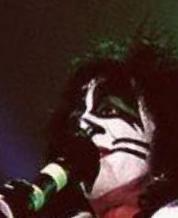
\includegraphics[width=0.25\textwidth]{1781334651982.png}
  \hfill
  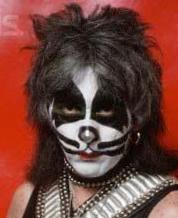
\includegraphics[width=0.25\textwidth]{1781335081362.png}
  \hfill
  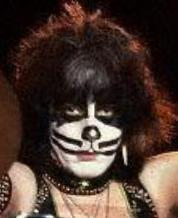
\includegraphics[width=0.25\textwidth]{1781335092626.png}
  \caption{identity\_07684 的注册集图片（MTCNN 均未检测到人脸）}
  \label{fig:celeba-fail-reg}
\end{figure}

\subsubsection{测试结果}

对 300 张测试图逐一处理：检测人脸、提取特征，与底库 99 类计算余弦相似度，取最相似的身份作为 Top-1 预测结果。由于 CelebA 数据集缺少逐脸标注文件，仅进行图片级评测，不进行逐脸级评测。不过 CelebA 的测试集基本为单人照，图片级评测可等价于逐脸评测。

\begin{table}[H]
\centering
\caption{CelebA 100 类图片级评测结果}
\label{tab:celeba-result}
\begin{tabular}{cc}
\toprule
指标 & 数值 \\
\midrule
总测试样本数 & 300 \\
正确识别数 & 292 \\
未检测到人脸 & 2 \\
Top-1 识别准确率 & \textbf{97.33\%} \\
\bottomrule
\end{tabular}
\end{table}

\subsubsection{成功样例}

\begin{table}[H]
\centering
\caption{CelebA 成功识别样例}
\label{tab:celeba-success}
\begin{tabular}{cccc}
\toprule
图片 & 真实身份 & 预测身份 & 余弦相似度 \\
\midrule
152524.jpg & identity\_00070 & identity\_00070 & 0.85 \\
154146.jpg & identity\_00070 & identity\_00070 & 0.89 \\
156907.jpg & identity\_00070 & identity\_00070 & 0.87 \\
001048.jpg & identity\_00212 & identity\_00212 & 0.81 \\
044372.jpg & identity\_00212 & identity\_00212 & 0.70 \\
\bottomrule
\end{tabular}
\end{table}

\subsubsection{失败样例分析}

\begin{table}[H]
\centering
\caption{CelebA 失败识别样例及原因分析}
\label{tab:celeba-fail}
\begin{tabular}{cccp{5cm}}
\toprule
图片 & 真实身份 & 预测身份 & 失败原因 \\
\midrule
042893.jpg & identity\_00503 & identity\_04198 & 测试图与注册图姿态差异大，模型将姿态相似的其他身份误判为更相似 \\
027259.jpg & identity\_01523 & unknown & 测试图光照条件与注册图差异显著，特征向量偏移较大 \\
171177.jpg & identity\_03565 & identity\_06360 & 测试图为侧脸，注册图均为正面，角度差异导致该样本特征不匹配 \\
082103.jpg & identity\_07684 & 未检测到人脸 & MTCNN 未检测到人脸，该身份的注册图同样无法检测 \\
\bottomrule
\end{tabular}
\end{table}

\begin{figure}[H]
  \centering
  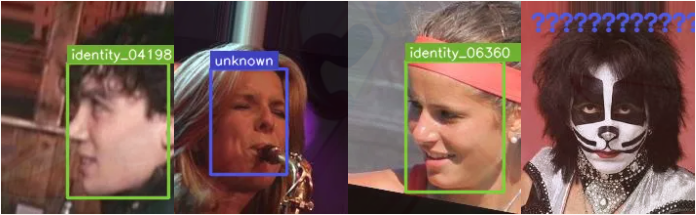
\includegraphics[width=0.85\textwidth]{1781367143450.png}
  \caption{CelebA 失败样例}
  \label{fig:celeba-fail}
\end{figure}

失败案例的共同特点：(1) 注册图与测试图在姿态、光照、遮挡等方面存在较大差异；(2) 个别身份的注册图质量不佳。(3) identity\_07684 的所有图片均无法被 MTCNN 检测到人脸，属于数据质量问题。

\subsection{自收集 20 类身份数据测试}

\subsubsection{测试设置}

使用自收集的 20 类公开人物数据，每人 2 张注册图、3 张测试图，共 100 张图片。测试集包含 20 张单人照和 40 张多人照。所有 20 类身份均成功注册。

\subsubsection{图片级评测结果}

\begin{table}[H]
\centering
\caption{自收集 20 类图片级评测结果}
\label{tab:custom-img-result}
\begin{tabular}{cc}
\toprule
指标 & 数值 \\
\midrule
总测试样本数 & 60 \\
正确识别数 & 60 \\
未检测到人脸 & 0 \\
Top-1 识别准确率 & \textbf{100.00\%} \\
\bottomrule
\end{tabular}
\end{table}

\subsubsection{逐脸级评测结果}

\begin{table}[H]
\centering
\caption{自收集 20 类逐脸级评测结果}
\label{tab:custom-face-result}
\begin{tabular}{cc}
\toprule
指标 & 数值 \\
\midrule
标注人脸总数 & 156 \\
正确识别人脸数 & 151 \\
逐脸准确率 & \textbf{96.79\%} \\
严格图片级准确率 & \textbf{93.33\%} \\
\bottomrule
\end{tabular}
\end{table}

图片级 100\% 与人脸级严格 93.33\% 的差异源于评测策略不同：图片级评测只需多人照中目标人物被正确匹配即可，而人脸级严格评测要求图中所有人脸都被正确识别。

\subsubsection{成功样例}

\begin{table}[H]
\centering
\caption{自收集 20 类成功识别样例}
\label{tab:custom-success}
\begin{tabular}{cccc}
\toprule
图片 & 真实身份 & 预测身份 & 余弦相似度 \\
\midrule
p01\_t01.jpg & p01（成龙） & p01 & 0.82 \\
p09\_t03.jpg & p09（马云） & p09 & 0.88 \\
p05\_t02.jpg & p05+p04 & p05+p04 & 0.76 / 0.74 \\
\bottomrule
\end{tabular}
\end{table}

\begin{figure}[H]
  \centering
  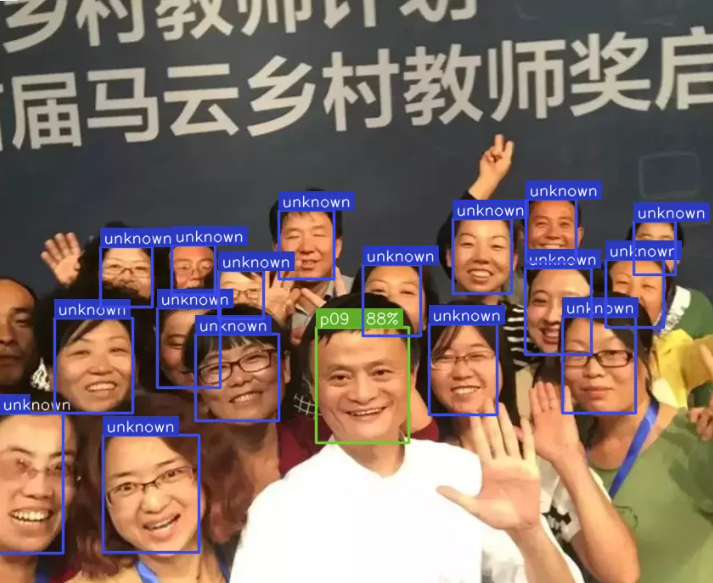
\includegraphics[width=0.7\textwidth]{1781367604327.png}
  \caption{自收集数据集多人照成功识别示例（p09 马云）}
  \label{fig:custom-success}
\end{figure}

\begin{figure}[H]
  \centering
  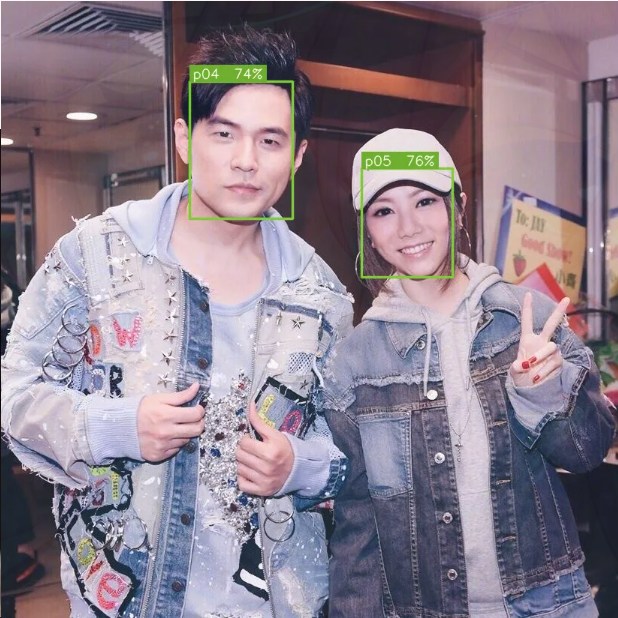
\includegraphics[width=0.7\textwidth]{1781367204484.png}
  \caption{自收集数据集多人照成功识别示例（p04 周杰伦 + p05 邓紫棋）}
  \label{fig:custom-success2}
\end{figure}

\subsubsection{失败样例分析}

图片级评测无失败案例（60/60），人脸级严格评测中有 5 张人脸识别失败（151/156）。失败分为两类：

\textbf{类型一：unknown 人脸被误判为已知身份。}多人照中非目标人员的人脸与底库中某身份的相似度超过阈值，导致系统输出错误身份。

\begin{figure}[H]
  \centering
  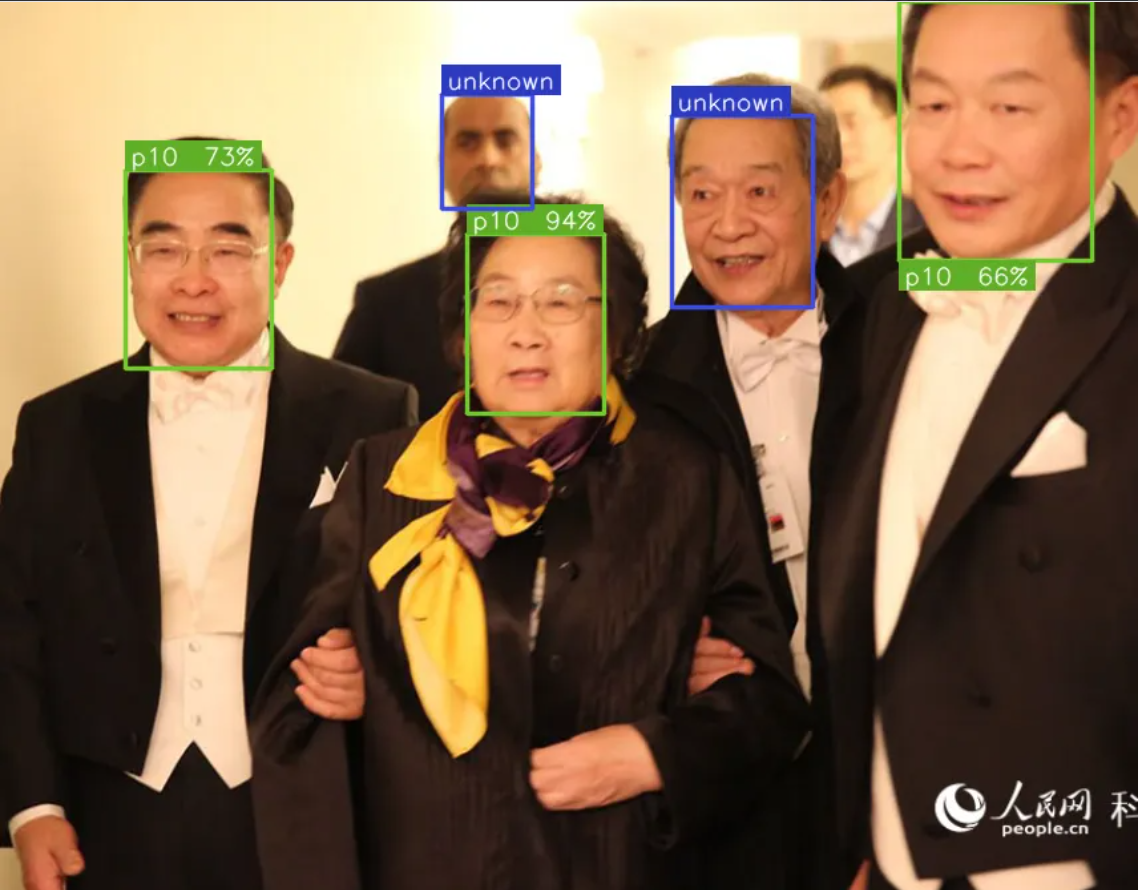
\includegraphics[width=0.5\textwidth]{1781367743328.png}
  \caption{unknown 人脸被误判为屠呦呦（相似度 0.66）}
  \label{fig:fail-type1}
\end{figure}

\textbf{类型二：目标人物被误判为 unknown。}目标人物的人脸因姿态、光照、遮挡等原因，与底库中自身身份的相似度低于阈值。

\begin{figure}[H]
  \centering
  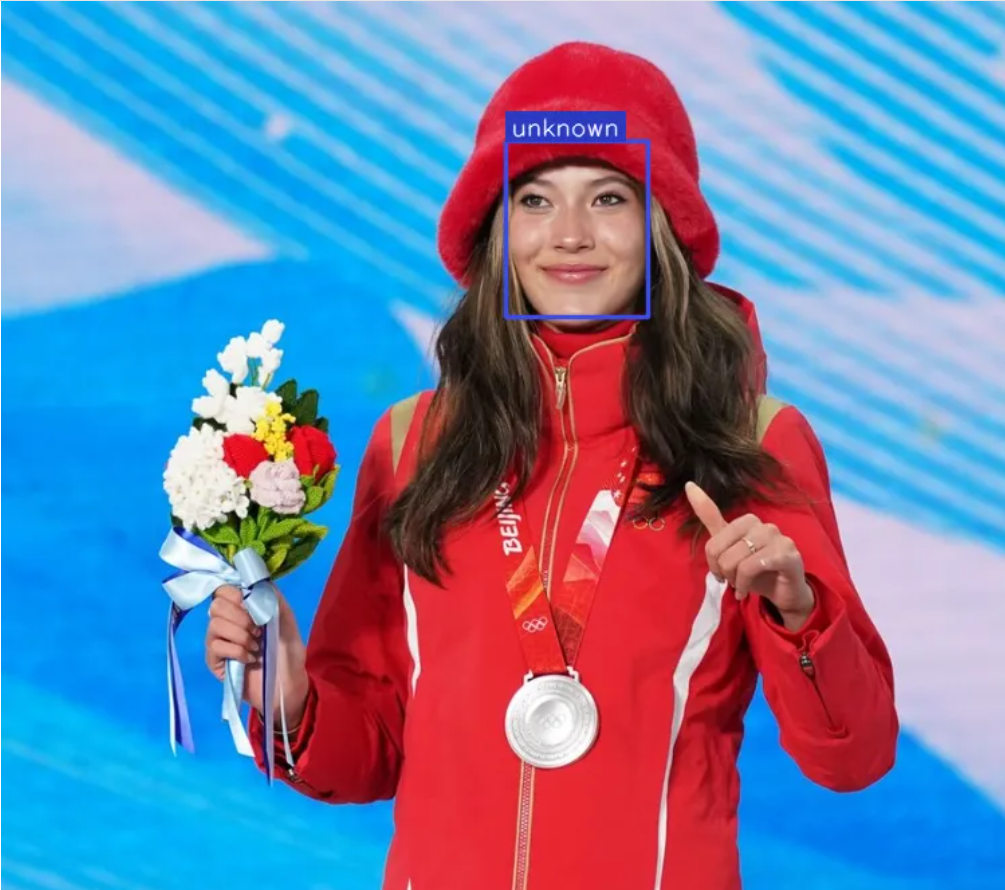
\includegraphics[width=0.45\textwidth]{1781368157336.png}
  \hfill
  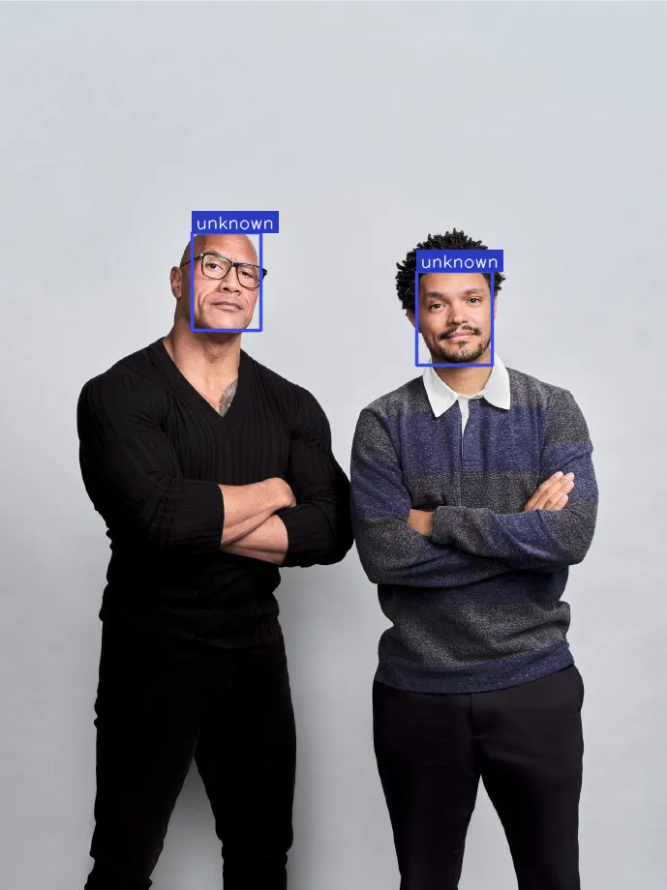
\includegraphics[width=0.45\textwidth]{1781368128585.png}
  \caption{目标人物被误判为 unknown：左为谷爱凌（相似度 0.58），右为 Dwayne Johnson（相似度 0.54）}
  \label{fig:fail-type2}
\end{figure}

\subsection{阈值灵敏度分析}
\label{sec:sensitivity}

为确定最优相似度阈值，在自收集 20 类数据集上对阈值进行灵敏度分析。阈值从 0.50 到 0.80 以步长 0.01 逐步扫描，记录每个阈值下的逐脸准确率、图片级严格准确率，以及两类错误数量（已知识别为未知、未知识别为已知）。

\begin{figure}[H]
  \centering
  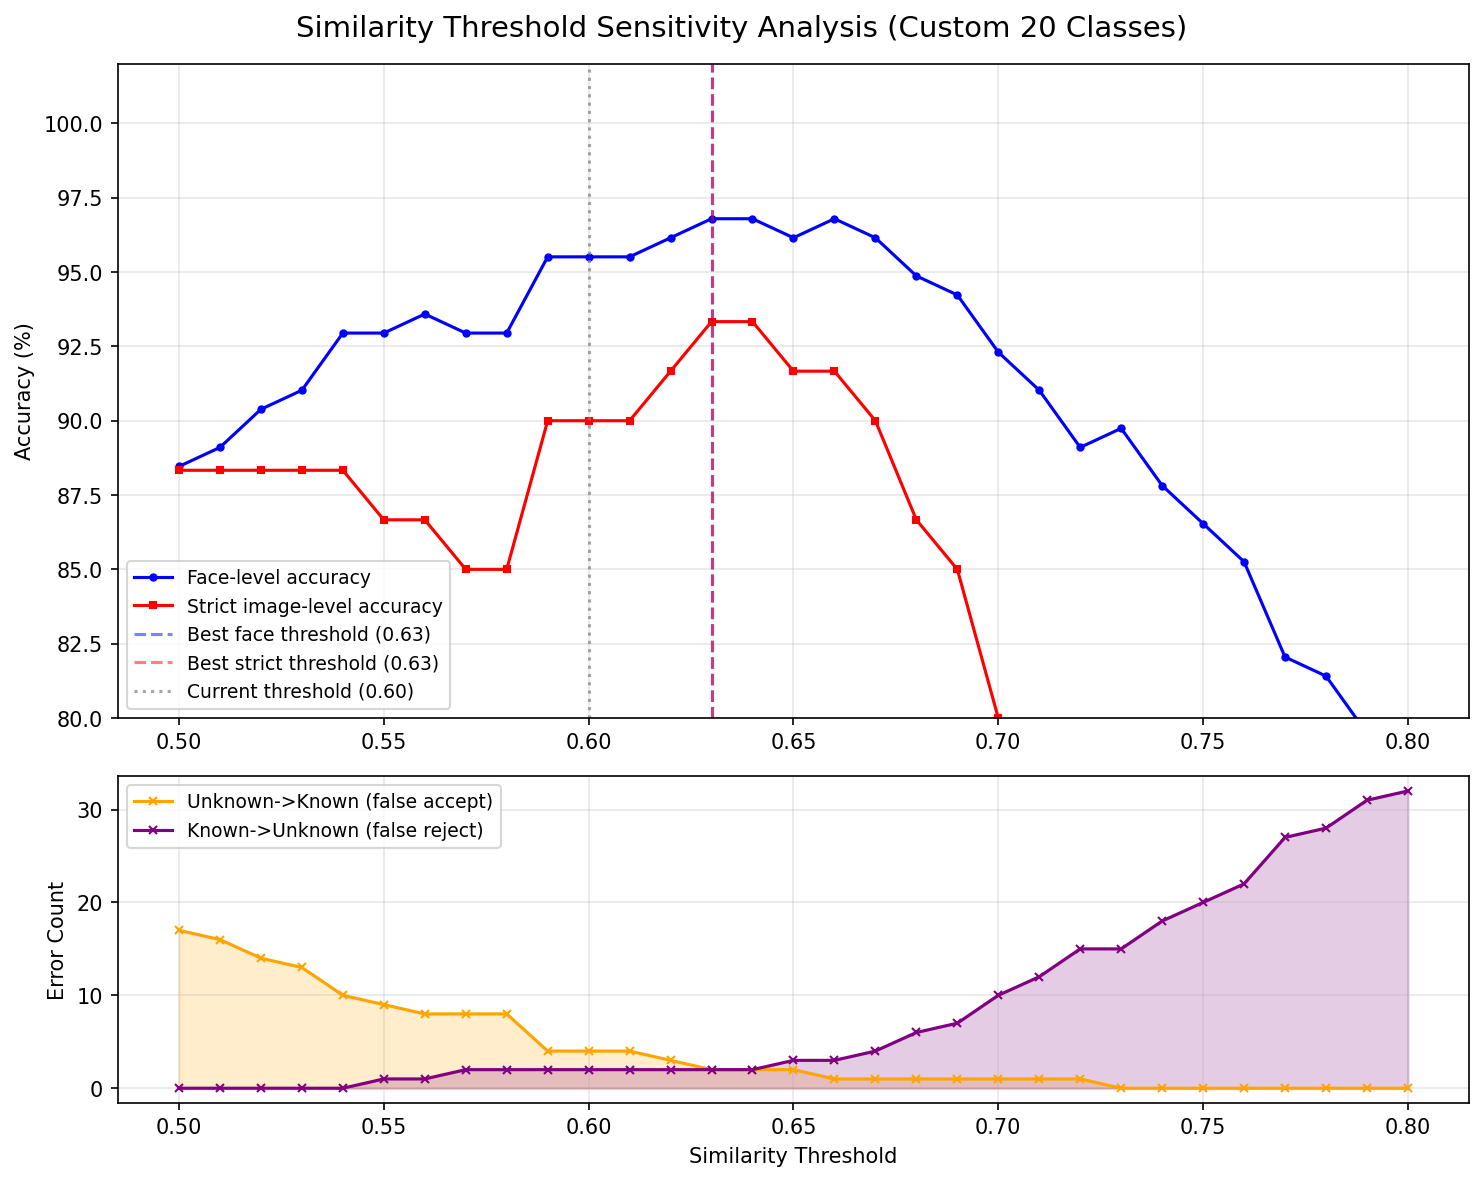
\includegraphics[width=0.85\textwidth]{1781366910403.png}
  \caption{相似度阈值灵敏度分析曲线}
  \label{fig:sensitivity}
\end{figure}

分析结果表明，当阈值取 0.63 时，图片级准确率与逐脸准确率均达到最大值，且识别错误的样本数最少（已知识别为未知和未知识别为已知的人脸数各为 2）。因此，最终采用 $\tau = 0.63$ 作为默认阈值。

\subsection{两种评测策略的对比}

表~\ref{tab:eval-compare} 对比了两种评测策略在数据集上的表现。

\begin{table}[H]
\centering
\caption{评测策略对比}
\label{tab:eval-compare}
\begin{tabular}{lccc}
\toprule
数据集 & 图片级 Top-1 & 逐脸准确率 & 图片级严格准确率 \\
\midrule
CelebA 100 类 & 97.33\% & --- & --- \\
自收集 20 类 & 100.00\% & 96.79\% & 93.33\% \\
\midrule
\multicolumn{4}{l}{\textit{任务要求基线：Top-1 $\geq$ 70\%}} \\
\bottomrule
\end{tabular}
\end{table}

两个数据集的 Top-1 准确率均达到 70\% 的基线要求。自收集数据集的图片级准确率达到 100\%，说明系统能够在各种场景下找到目标人物。逐脸准确率略低于图片级，主要受到多人照中非目标人员误判的影响。


% ======== 第五章 ========
\section{前端可视化展示}

\subsection{界面功能}

前端功能包括：

\begin{itemize}
  \item \textbf{图片上传}：支持拖拽上传或点击选择图片；
  \item \textbf{底库切换}：提供三个选项，可选择 CelebA 100 类底库、自收集 20 类底库或全部 120 类底库（无此需求）；
  \item \textbf{实时识别}：点击"开始识别"按钮后，系统完成人脸检测、特征提取、底库比对，返回标注后的图片和识别结果；
  \item \textbf{结果可视化}：已知身份用绿色矩形框标注，显示身份编号和置信度百分比；未知身份用红色矩形框标注，显示 \texttt{unknown}。
\end{itemize}

\subsection{界面截图}

\begin{figure}[H]
  \centering
  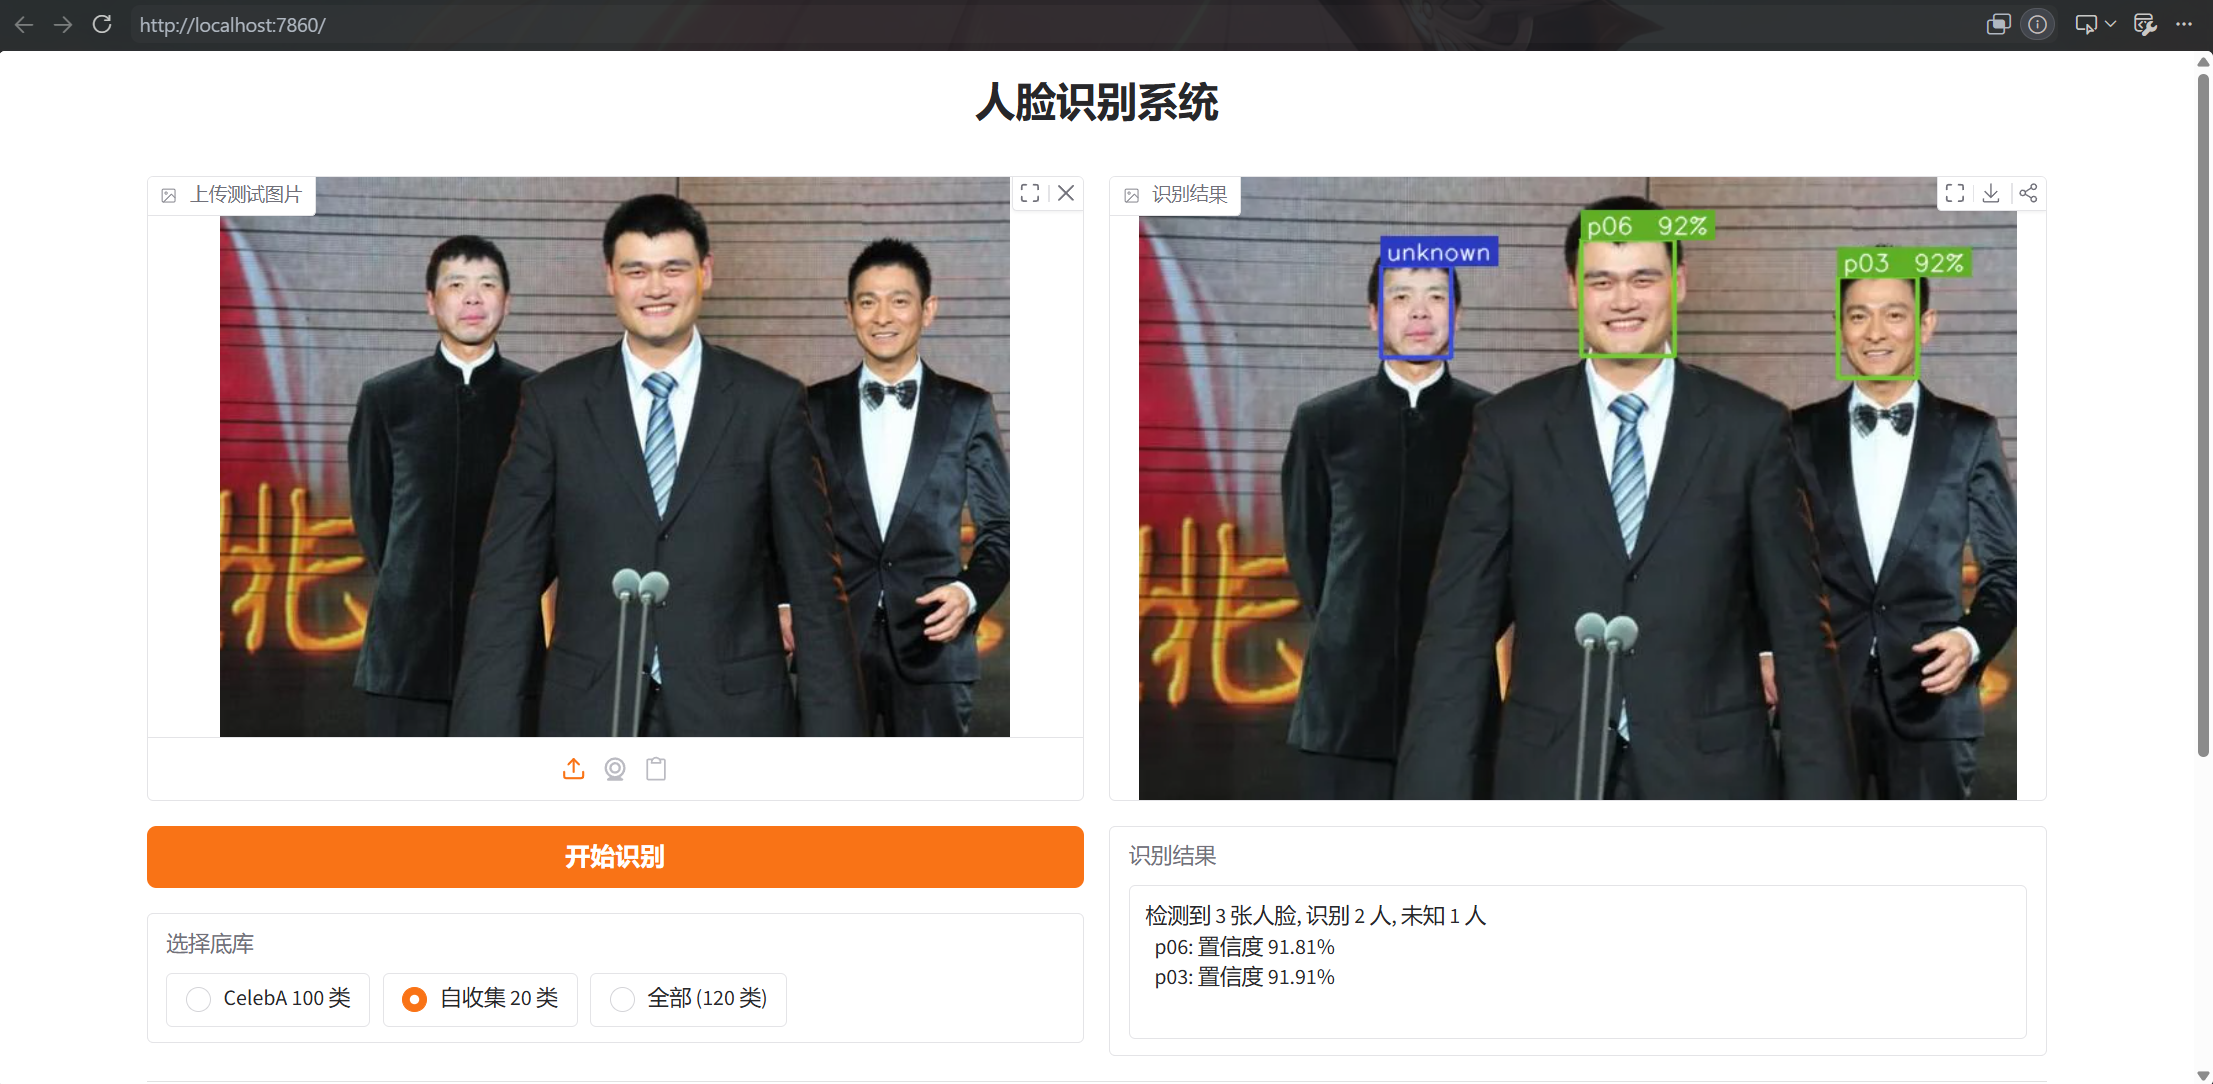
\includegraphics[width=0.85\textwidth]{1781368281763.png}
  \caption{Gradio Web 演示界面截图}
  \label{fig:gradio}
\end{figure}

界面布局说明：
\begin{itemize}
  \item 左侧为输入区域：图片上传框 + "开始识别"按钮；
  \item 右侧为输出区域：识别结果图片 + 识别结果文字（检测到的人脸数、识别出的身份、置信度）；
  \item 底部显示系统信息：运行设备、所用模型、特征模型、相似度阈值。
\end{itemize}

\subsection{运行方式}

启动命令：
\begin{lstlisting}[language={}, caption={启动 Gradio 服务}, label={lst:gradio-start}]
python app.py
# 浏览器访问 http://localhost:7860
\end{lstlisting}


% ======== 第六章 ========
\section{总结与展望}

\subsection{系统完成情况}

本系统完成了人脸识别系统的全部核心功能，完成情况如表~\ref{tab:completion} 所示。

\begin{table}[H]
\centering
\caption{系统任务完成情况}
\label{tab:completion}
\begin{tabular}{p{4cm}cp{5.5cm}}
\toprule
任务要求 & 完成情况 & 达成指标 \\
\midrule
本地运行，不调用云端 API & \checkmark & 全部模型推理在本地 GPU 执行 \\
数据收集与标注 & \checkmark & 20 类身份，注册集 40 张，测试集 60 张 \\
CelebA数据集 100 类测试 & \checkmark & Top-1 准确率 97.33\%（要求 $\geq$ 70\%） \\
自收集 20 类测试 & \checkmark & Top-1 准确率 100.00\%（要求 $\geq$ 70\%） \\
前端演示 & \checkmark & Gradio Web 界面，支持图片上传、底库切换 \\
\bottomrule
\end{tabular}
\end{table}

\subsection{主要不足}

\begin{enumerate}
  \item \textbf{MTCNN 检测效果：}部分图片（如 CelebA 的 identity\_07684）MTCNN 无法检测到人脸, 部分图片将不是人脸的区域误识别为人脸。
  \item \textbf{注册集规模小：}自收集数据每人仅 2 张注册图，特征向量的多样性不足。当测试图与注册图在姿态、光照等方面差异较大时，很容易出现匹配失败。
  \item \textbf{阈值固定：}相似度阈值为统一设置，未针对不同身份的特点进行个性化调整。部分身份的类内方差较大（如同一人的不同照片差异大），需要更低的阈值；部分类间方差较小（如长相相似的不同人），需要更高的阈值。
  \item \textbf{无学习和扩展能力：}采用静态底库，无法动态调整特征向量或新增身份。
\end{enumerate}

\subsection{改进方向}

\begin{enumerate}
  \item \textbf{替换检测器：}使用 RetinaFace 或 SCRFD 等更先进的人脸检测器替代 MTCNN，提升小脸、侧脸、遮挡人脸的检测率。
  \item \textbf{使用更强的特征模型：}采用 ArcFace\cite{deng2019arcface} 或 AdaFace 等方法训练的模型，通过改进损失函数提升特征的判别能力。
  \item \textbf{增加注册图数量：}每人收集 5--10 张注册图，覆盖不同姿态（正面、左侧、右侧）、不同光照（自然光、室内光、逆光）、不同表情（笑脸、严肃），提升底库特征的鲁棒性。
  \item \textbf{数据增强：}对注册图进行随机水平翻转、颜色抖动、随机裁剪等数据增强操作，人工扩充注册集的多样性。
  \item \textbf{自适应阈值：}根据每个身份的类内特征方差动态调整阈值，对方差大的身份使用更低的阈值，对方差小的身份使用更高的阈值。
\end{enumerate}


% ======== 参考文献 ========
\newpage
\begin{thebibliography}{9}

\bibitem{zhang2016mtcnn}
Zhang, K., Zhang, Z., Li, Z., \& Qiao, Y. (2016).
Joint Face Detection and Alignment Using Multitask Cascaded Convolutional Networks.
\textit{IEEE Signal Processing Letters}, 23(10), 1499--1503.

\bibitem{schroff2015facenet}
Schroff, F., Kalchenko, D., \& Philbin, J. (2015).
FaceNet: A Unified Embedding for Face Recognition and Clustering.
\textit{Proceedings of the IEEE Conference on Computer Vision and Pattern Recognition (CVPR)}, 815--823.

\bibitem{deng2019arcface}
Deng, J., Guo, J., Xue, N., \& Zafeiriou, S. (2019).
ArcFace: Additive Angular Margin Loss for Deep Face Recognition.
\textit{Proceedings of the IEEE/CVF Conference on Computer Vision and Pattern Recognition (CVPR)}, 4690--4699.

\bibitem{cao2018vggface2}
Cao, Q., Shen, L., Xie, W., Parkhi, O. M., \& Zisserman, A. (2018).
VGGFace2: A Dataset for Recognising Faces across Pose and Age.
\textit{IEEE International Conference on Automatic Face \& Gesture Recognition (FG)}, 67--74.

\bibitem{liu2015celeba}
Liu, Z., Luo, P., Wang, X., \& Tang, X. (2015).
Deep Learning Face Attributes in the Wild.
\textit{Proceedings of the IEEE International Conference on Computer Vision (ICCV)}, 3730--3738.

\bibitem{celeba_url}
CelebA 数据集. \url{https://mmlab.ie.cuhk.edu.hk/projects/CelebA.html}

\bibitem{facenet_pytorch}
facenet-pytorch 库. \url{https://github.com/timesler/facenet-pytorch}

\bibitem{gradio_url}
Gradio 文档. \url{https://www.gradio.app/}

\end{thebibliography}

\end{document}
